\documentclass[dvipsnames,tikz]{standalone}
\usepackage{amsmath}
\usepackage{arevmath}
\usepackage{xcolor}
\usepackage{tikz}
\usetikzlibrary{calc}
\usetikzlibrary{decorations.pathreplacing,calligraphy,3d}
\usepackage{tikz-3dplot} 

\tikzset{main/.style={thick, circle, color=black}}

\newcommand{\arrowIn}{
	\tikz \draw[-stealth] (-1pt,0) -- (1pt,0);
}

\begin{document}
	
	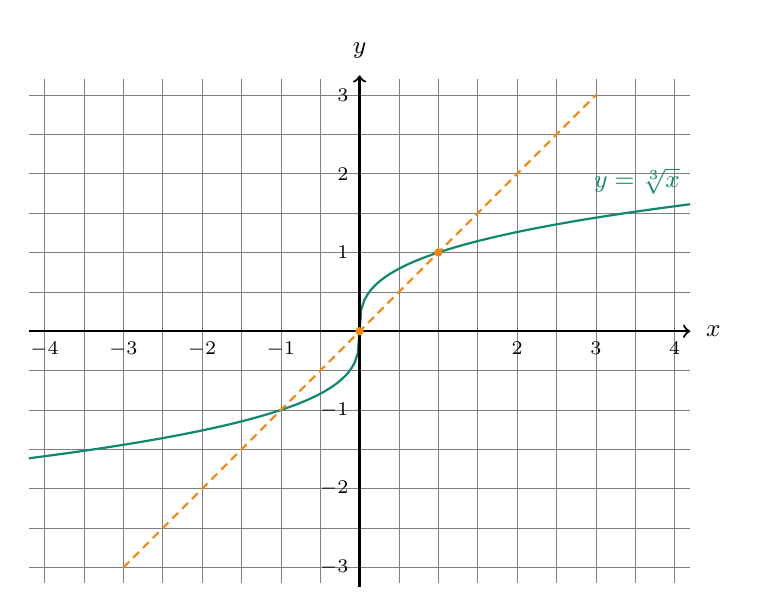
\begin{tikzpicture}[font=\small, tl/.style = {black, inner sep=1pt, font=\scriptsize} ]
		% grid
		\draw[main, very thin, xstep=0.5, ystep=0.5, semitransparent] (-4.2,-3.2) grid (4.2,3.2);
		
		% y tick label
		\foreach \y in {-3,-2,-1,1,2,3}{
			\node[tl,left=1mm] at (0,\y) {$\y$};
		}
		% x tick label
		\foreach \x in {-4,-3,-2,-1,2,3,4}{
			\node[tl,below=1mm] at (\x,0) {$\x$};
		}
		
		% curve
		\draw[thick,PineGreen,domain=-4.2:4.2,variable=\x, samples=200] plot(\x,{(\x^(1/3)}) node [above left] {$y=\sqrt[3]{x}$};
		
		% axes
		\draw[main, ->,thick] (-4.2,0) -- (4.2,0) node[right] {$x$};
		\draw[main, ->,thick] (0,-3.25) -- (0, 3.25) node[above] {$y$};	
		
		\fill[BurntOrange] (0,0) circle (1.5pt);
		\fill[BurntOrange] (1,1) circle (1.5pt);
		\draw[thick, densely dashed,BurntOrange,domain=-3:3,variable=\x] plot(\x,{\x});
	\end{tikzpicture}
	
	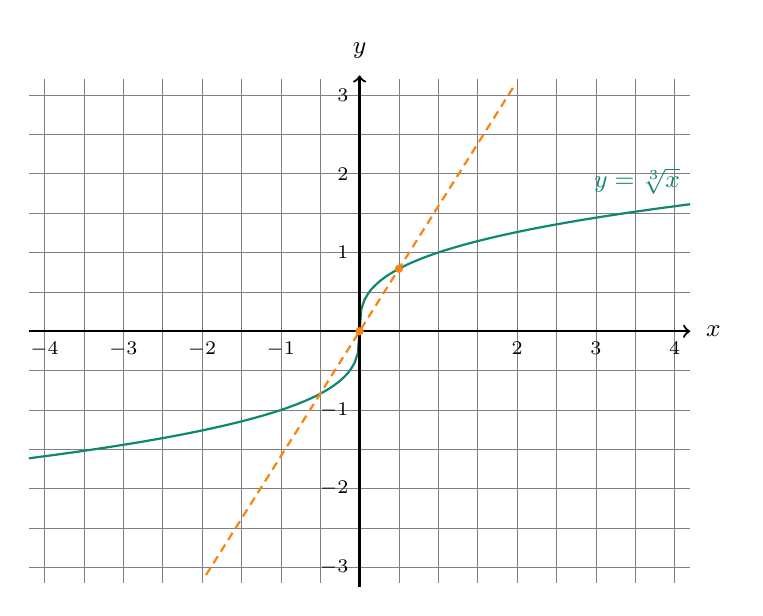
\begin{tikzpicture}[font=\small, tl/.style = {black, inner sep=1pt, font=\scriptsize} ]
		% grid
		\draw[main, very thin, xstep=0.5, ystep=0.5, semitransparent] (-4.2,-3.2) grid (4.2,3.2);
		
		% y tick label
		\foreach \y in {-3,-2,-1,1,2,3}{
			\node[tl,left=1mm] at (0,\y) {$\y$};
		}
		% x tick label
		\foreach \x in {-4,-3,-2,-1,2,3,4}{
			\node[tl,below=1mm] at (\x,0) {$\x$};
		}
		
		% curve
		\draw[thick,PineGreen,domain=-4.2:4.2,variable=\x, samples=200] plot(\x,{(\x^(1/3)}) node [above left] {$y=\sqrt[3]{x}$};
		
		% axes
		\draw[main, ->,thick] (-4.2,0) -- (4.2,0) node[right] {$x$};
		\draw[main, ->,thick] (0,-3.25) -- (0, 3.25) node[above] {$y$};	
		
		\fill[BurntOrange] (0,0) circle (1.5pt);
		\fill[BurntOrange] (0.5,0.79370053) circle (1.5pt);
		\draw[thick, densely dashed,BurntOrange,domain=-1.95:1.95,variable=\x] plot(\x,{1.5874010519682*\x});
	\end{tikzpicture}
	
	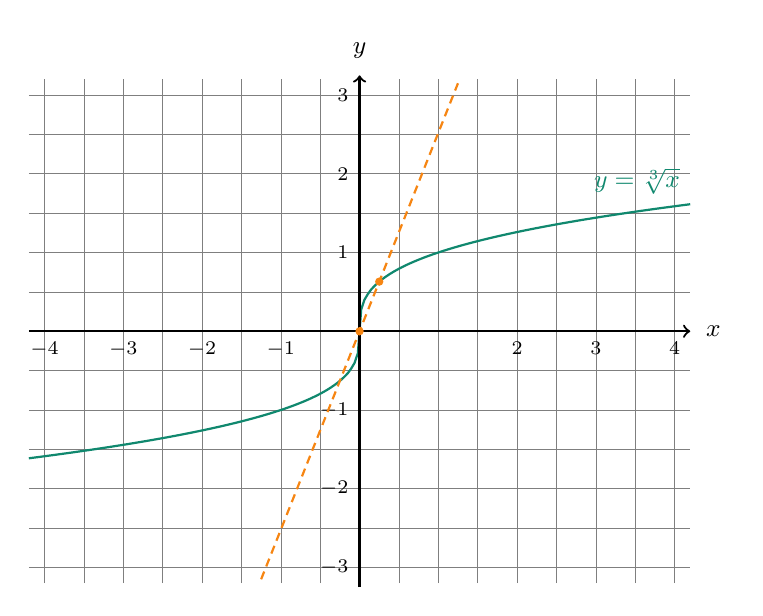
\begin{tikzpicture}[font=\small, tl/.style = {black, inner sep=1pt, font=\scriptsize} ]
		% grid
		\draw[main, very thin, xstep=0.5, ystep=0.5, semitransparent] (-4.2,-3.2) grid (4.2,3.2);
		
		% y tick label
		\foreach \y in {-3,-2,-1,1,2,3}{
			\node[tl,left=1mm] at (0,\y) {$\y$};
		}
		% x tick label
		\foreach \x in {-4,-3,-2,-1,2,3,4}{
			\node[tl,below=1mm] at (\x,0) {$\x$};
		}
		
		% curve
		\draw[thick,PineGreen,domain=-4.2:4.2,variable=\x, samples=200] plot(\x,{(\x^(1/3)}) node [above left] {$y=\sqrt[3]{x}$};
		
		% axes
		\draw[main, ->,thick] (-4.2,0) -- (4.2,0) node[right] {$x$};
		\draw[main, ->,thick] (0,-3.25) -- (0, 3.25) node[above] {$y$};	
		
		\fill[BurntOrange] (0,0) circle (1.5pt);
		\fill[BurntOrange] (0.25,0.62996052) circle (1.5pt);
		\draw[thick, densely dashed,BurntOrange,domain=-1.25:1.25,variable=\x] plot(\x,{2.519842099789746*\x});
	\end{tikzpicture}
	
	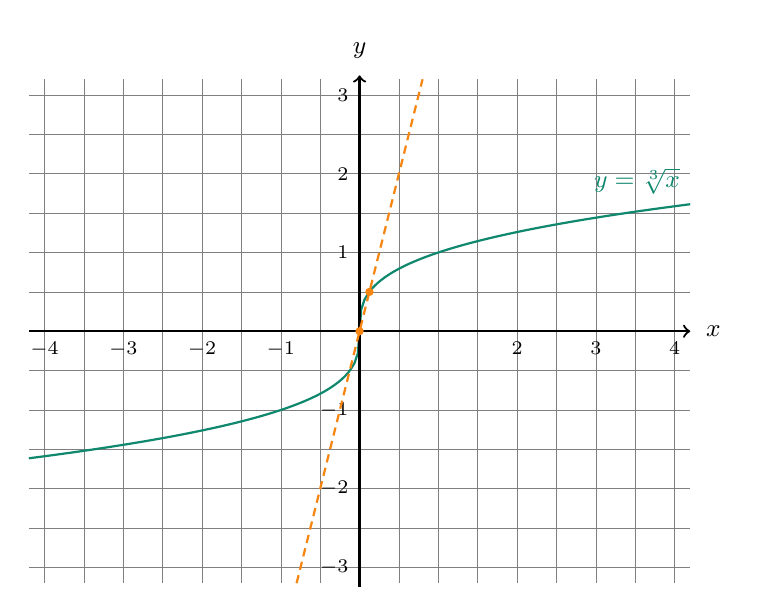
\begin{tikzpicture}[font=\small, tl/.style = {black, inner sep=1pt, font=\scriptsize} ]
		% grid
		\draw[main, very thin, xstep=0.5, ystep=0.5, semitransparent] (-4.2,-3.2) grid (4.2,3.2);
		
		% y tick label
		\foreach \y in {-3,-2,-1,1,2,3}{
			\node[tl,left=1mm] at (0,\y) {$\y$};
		}
		% x tick label
		\foreach \x in {-4,-3,-2,-1,2,3,4}{
			\node[tl,below=1mm] at (\x,0) {$\x$};
		}
		
		% curve
		\draw[thick,PineGreen,domain=-4.2:4.2,variable=\x, samples=200] plot(\x,{(\x^(1/3)}) node [above left] {$y=\sqrt[3]{x}$};
		
		% axes
		\draw[main, ->,thick] (-4.2,0) -- (4.2,0) node[right] {$x$};
		\draw[main, ->,thick] (0,-3.25) -- (0, 3.25) node[above] {$y$};	
		
		\fill[BurntOrange] (0,0) circle (1.5pt);
		\fill[BurntOrange] (0.125,0.5) circle (1.5pt);
		\draw[thick, densely dashed,BurntOrange,domain=-0.8:0.8,variable=\x] plot(\x,{4.0*\x});
	\end{tikzpicture}
	
	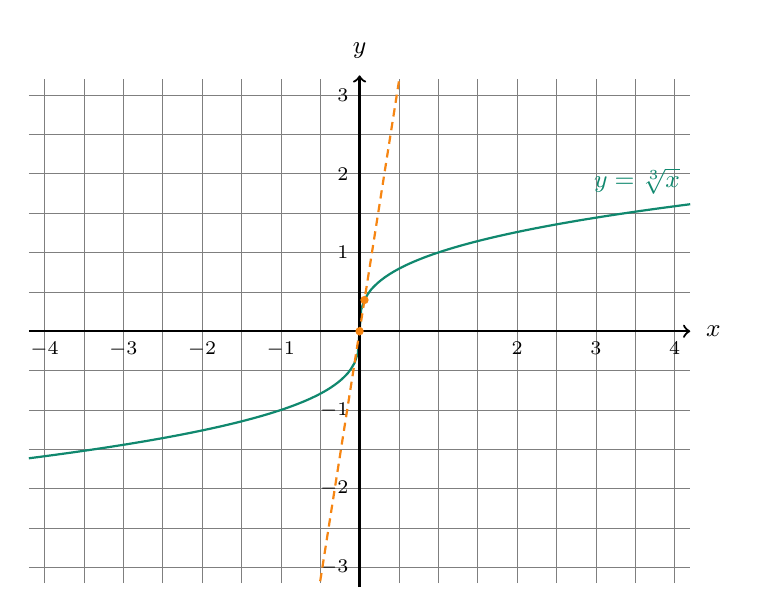
\begin{tikzpicture}[font=\small, tl/.style = {black, inner sep=1pt, font=\scriptsize} ]
		% grid
		\draw[main, very thin, xstep=0.5, ystep=0.5, semitransparent] (-4.2,-3.2) grid (4.2,3.2);
		
		% y tick label
		\foreach \y in {-3,-2,-1,1,2,3}{
			\node[tl,left=1mm] at (0,\y) {$\y$};
		}
		% x tick label
		\foreach \x in {-4,-3,-2,-1,2,3,4}{
			\node[tl,below=1mm] at (\x,0) {$\x$};
		}
		
		% curve
		\draw[thick,PineGreen,domain=-4.2:4.2,variable=\x, samples=200] plot(\x,{(\x^(1/3)}) node [above left] {$y=\sqrt[3]{x}$};
		
		% axes
		\draw[main, ->,thick] (-4.2,0) -- (4.2,0) node[right] {$x$};
		\draw[main, ->,thick] (0,-3.25) -- (0, 3.25) node[above] {$y$};	
		
		\fill[BurntOrange] (0,0) circle (1.5pt);
		\fill[BurntOrange] (0.0625,0.39685026) circle (1.5pt);
		\draw[thick, densely dashed,BurntOrange,domain=-0.5:0.5,variable=\x] plot(\x,{6.3496*\x});
	\end{tikzpicture}
	
	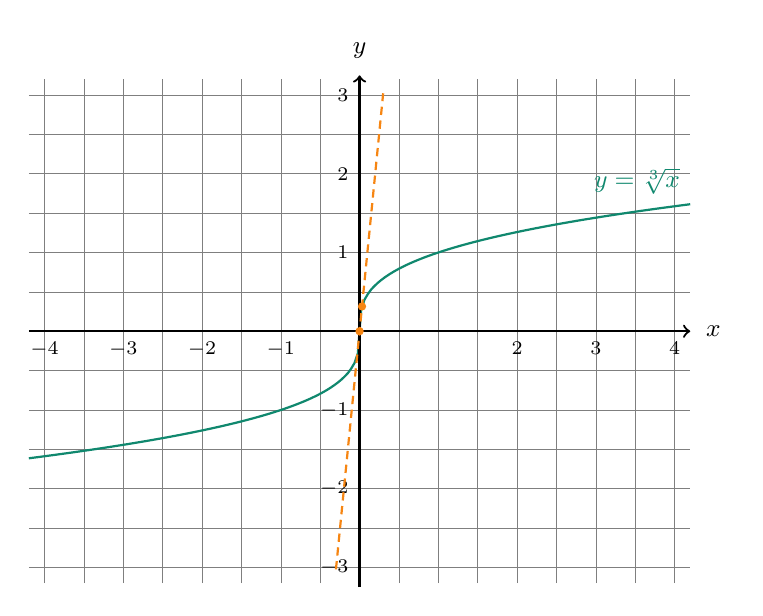
\begin{tikzpicture}[font=\small, tl/.style = {black, inner sep=1pt, font=\scriptsize} ]
		% grid
		\draw[main, very thin, xstep=0.5, ystep=0.5, semitransparent] (-4.2,-3.2) grid (4.2,3.2);
		
		% y tick label
		\foreach \y in {-3,-2,-1,1,2,3}{
			\node[tl,left=1mm] at (0,\y) {$\y$};
		}
		% x tick label
		\foreach \x in {-4,-3,-2,-1,2,3,4}{
			\node[tl,below=1mm] at (\x,0) {$\x$};
		}
		
		% curve
		\draw[thick,PineGreen,domain=-4.2:4.2,variable=\x, samples=200] plot(\x,{(\x^(1/3)}) node [above left] {$y=\sqrt[3]{x}$};
		
		% axes
		\draw[main, ->,thick] (-4.2,0) -- (4.2,0) node[right] {$x$};
		\draw[main, ->,thick] (0,-3.25) -- (0, 3.25) node[above] {$y$};	
		
		\fill[BurntOrange] (0,0) circle (1.5pt);
		\fill[BurntOrange] (0.03125,0.31498026) circle (1.5pt);
		\draw[thick, densely dashed,BurntOrange,domain=-0.3:0.3,variable=\x] plot(\x,{10.0793*\x});
	\end{tikzpicture}
\end{document}